% AgonProject poster — AIG tikzposter style (A0 portrait)
% Screenshot-showcase layout. Style reused from the AIG sample poster;
% the previous sample content is preserved in sample_poster.tex.bak.

\documentclass[25pt,a0paper,portrait,margin=2mm, innermargin=16mm, blockverticalspace=6mm, colspace=15mm, subcolspace=10mm]{tikzposter}

\usepackage{aigpostersettings}

\usepackage{anyfontsize}
\usepackage{palatino}
\usepackage[utf8]{inputenc}
\usepackage[T1]{fontenc}
\usepackage{booktabs}
\usepackage[table]{xcolor}
\usepackage{graphicx}
\usepackage{amssymb,amsthm,amsmath,amsfonts}
\usepackage{qrcode}

% Local macros (kept minimal, no dependency on paper _macros.sty)
\newcommand{\agon}{\textsc{AgonProject}\xspace}
\newcommand{\tweety}{\textsc{TweetyProject}\xspace}
\providecommand{\xspace}{\ }

\usetitlestyle{aigpostertitle1}

\title{\parbox{0.95\linewidth}{{\fontsize{4cm}{4.2cm}\selectfont AgonProject}\\[0.5em]
    {\LARGE\normalfont\itshape An online platform for exploring approaches to formal argumentation}}}
%\author{Lars Bengel \quad Matti Berthold \quad Oleksandr Dzhychko \quad Matthias Thimm}
\institute{Artificial Intelligence Group, University of Hagen, Germany}

\usecolorstyle{aigpostercolor}
\usebackgroundstyle{aigposterback}
\useblockstyle{aigposterblockB}

\begin{document}

\maketitle

%======================================================================
% Row 1 — Motivation + live QR
%======================================================================
\begin{columns}
\column{1.0}
\useblockstyle{aigposterblockY}
\block{Why AgonProject?}{
    \begin{minipage}[t]{0.62\linewidth}
        \vspace*{0pt}
        Formal argumentation offers a rich \emph{zoo} of formalisms for reasoning with
        conflicting information --- but their diverse semantics, algorithms, and
        implementation details make them hard for students and newcomers to grasp.

        \vspace{0.6ex}
        \tweety provides the most comprehensive collection of argumentation
        implementations available, yet exposes only \emph{text-based} interfaces for a
        handful of tasks.

        \vspace{1.0ex}
        \yellowhighlight{\parbox{0.96\linewidth}{\vspace{0.4ex}
        \textbf{Goal:} a unified, \textbf{visual}, install-free web interface to
        \emph{construct}, \emph{evaluate}, and \emph{compare} argumentation formalisms
        --- right in the browser.\vspace{0.4ex}}}

        \vspace{1.0ex}
        Built with Vue 3 + TypeScript (client-side single-page app); reasoning tasks are
        delegated to a \tweety REST backend. Open source under GPL-3.0.
    \end{minipage}
    \hfill
    \begin{minipage}[t]{0.33\linewidth}
        \vspace*{0pt}
        \centering
        \colorlet{innerblocktitlebgcolor}{aigblue}
        \colorlet{innerblocktitlefgcolor}{white}
        \colorlet{innerblockbodybgcolor}{white}
        \colorlet{innerblockbodyfgcolor}{black}
        \innerblock{Try it now --- no installation}{
            \centering
            \qrcode[height=5cm]{http://agon.tweetyproject.org}\\[0.6ex]
            {\Large\bfseries\color{aigblue}\texttt{agon.tweetyproject.org}}
        }
    \end{minipage}
}\useblockstyle{aigposterblockB}
\end{columns}

%======================================================================
% Row 2 — Landing page + six formalisms
%======================================================================
\begin{columns}
\column{1.0}
\block{One Platform --- Six Argumentation Formalisms}{
    \begin{minipage}[c]{0.42\linewidth}
        \centering
        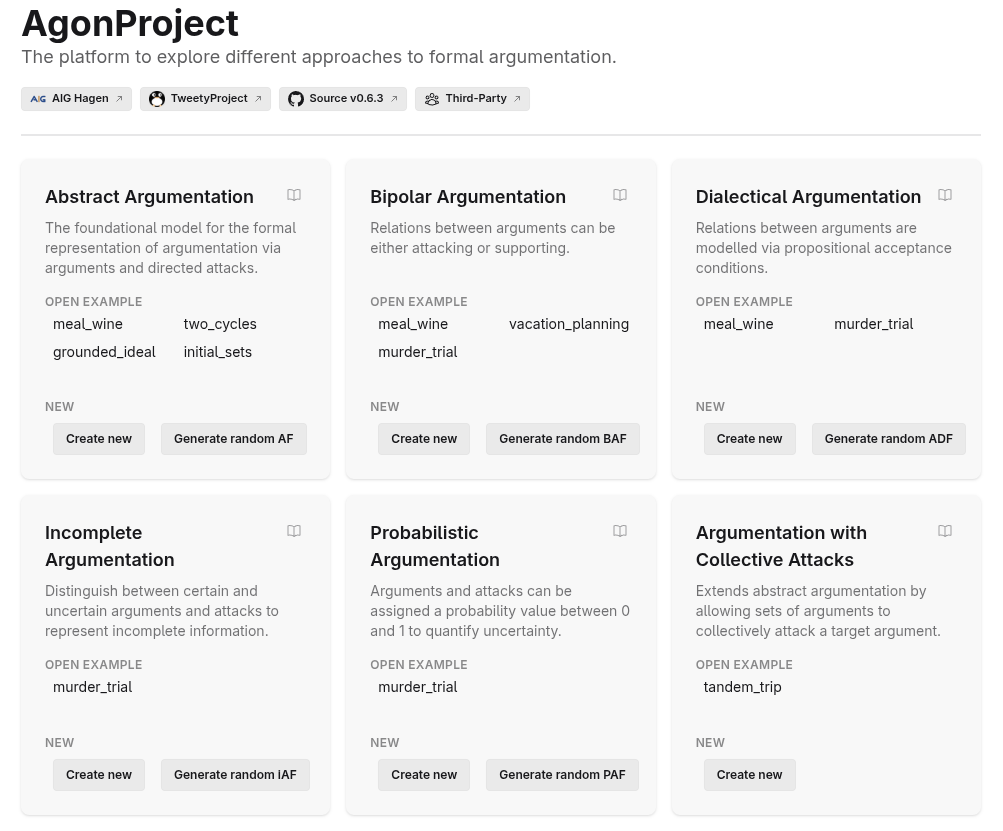
\includegraphics[width=0.90\linewidth]{figures/screenshot-landing.png}
    \end{minipage}
    \hfill
    \begin{minipage}[c]{0.54\linewidth}
        \begin{description}\setlength{\itemsep}{0.7ex}
            \item[AF] \emph{Abstract} argumentation --- arguments and directed attacks (Dung).
            \item[BAF] \emph{Bipolar} --- attacks \textbf{and} a support relation.
            \item[ADF] \emph{Abstract dialectical} --- propositional acceptance conditions.
            \item[iAF] \emph{Incomplete} --- uncertain arguments and attacks.
            \item[PAF] \emph{Probabilistic} --- probabilities on arguments and attacks.
            \item[SetAF] \emph{Collective attacks} --- sets of arguments attack a target.
        \end{description}
        \vspace{0.6ex}
        Every formalism shares the same editor, evaluation, export, generation, and
        learning features below --- so comparing them is effortless.
    \end{minipage}
}
\end{columns}

%======================================================================
% Row 3 — Core features
%======================================================================
\begin{columns}
\column{1.0}
\useblockstyle{aigposterblockY}
\block{What You Can Do}{
    \colorlet{innerblocktitlebgcolor}{aigblue}
    \colorlet{innerblocktitlefgcolor}{white}
    \colorlet{innerblockbodybgcolor}{white}
    \colorlet{innerblockbodyfgcolor}{black}
    \begin{minipage}[t]{0.185\linewidth}
        \innerblock{Build}{Interactive graph editor with directed, circular, radial and
        force-directed layouts (Graphviz) plus a physics simulation.}
    \end{minipage}\hfill
    \begin{minipage}[t]{0.185\linewidth}
        \innerblock{Evaluate}{Extension- and ranking-based semantics; credulous / sceptical
        acceptance; highlight extensions directly in the graph; compare in parallel windows.}
    \end{minipage}\hfill
    \begin{minipage}[t]{0.185\linewidth}
        \innerblock{Export \& Share}{One-click \LaTeX{} (\texttt{argumentation} package),
        SVG, TGF, and ICCMA AF-format --- plus a shareable URL.}
    \end{minipage}\hfill
    \begin{minipage}[t]{0.185\linewidth}
        \innerblock{Generate}{Random frameworks from eight \texttt{networkX} generators
        (Erd\H{o}s--R\'enyi, Watts--Strogatz, Barab\'asi--Albert, \dots).}
    \end{minipage}\hfill
    \begin{minipage}[t]{0.185\linewidth}
        \innerblock{Learn}{10+ step-by-step tutorials, an extensive glossary with literature
        references, and curated example frameworks.}
    \end{minipage}
}\useblockstyle{aigposterblockB}
\end{columns}

%======================================================================
% Row 4 — In action (three screenshots)
%======================================================================
\begin{columns}
\column{1.0}
\block{In Action}{
    \begin{minipage}[t]{0.325\linewidth}
        \centering
        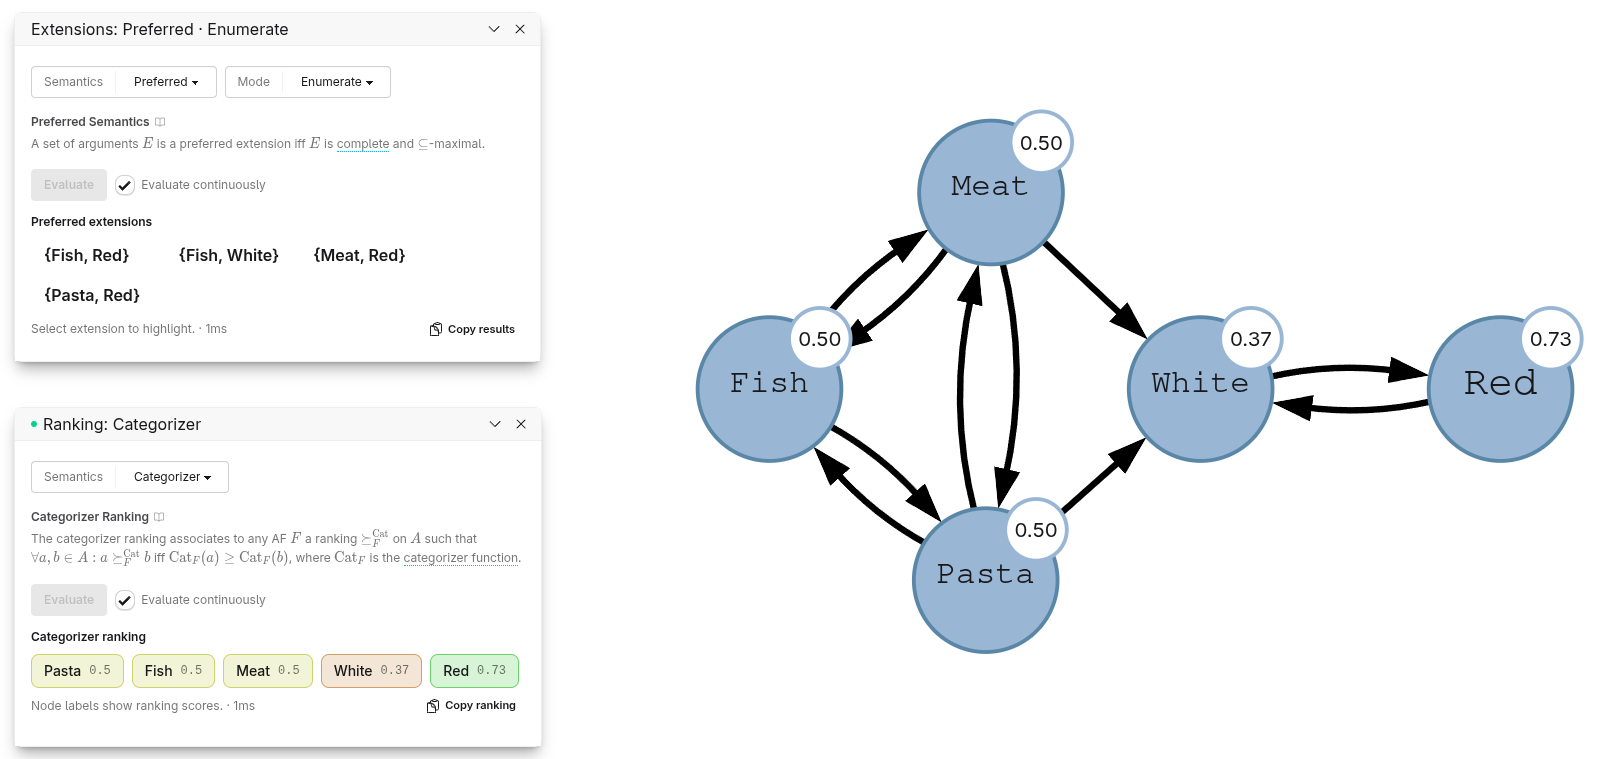
\includegraphics[width=0.93\linewidth]{figures/screenshot-af.png}\\[0.6ex]
        \raggedright\footnotesize
        \textbf{Evaluate \& rank (AF).} Preferred extensions are enumerated while the
        \emph{categoriser} ranking is annotated directly on each argument; evaluation
        windows can stay open in parallel.
    \end{minipage}\hfill
    \begin{minipage}[t]{0.325\linewidth}
        \centering
        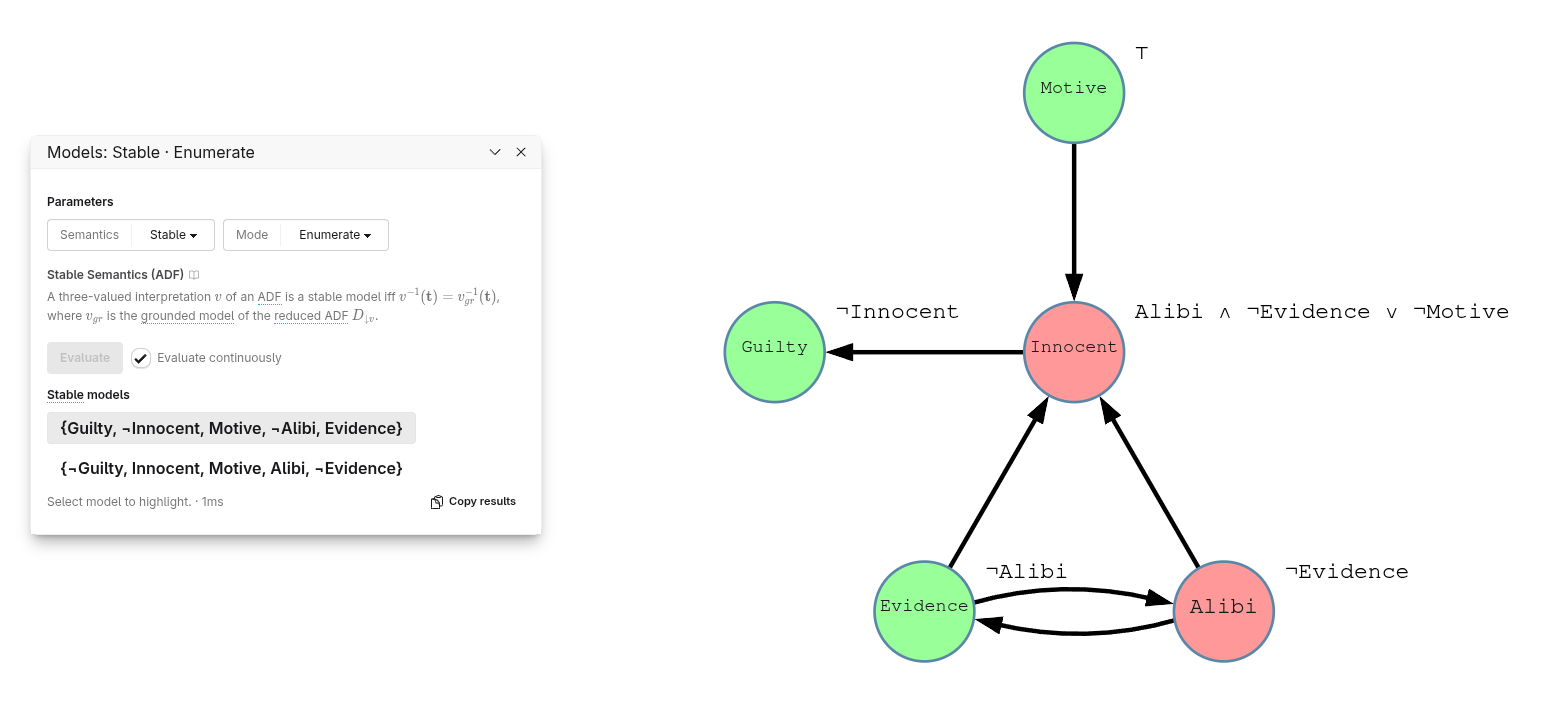
\includegraphics[width=0.93\linewidth]{figures/screenshot-adf.png}\\[0.6ex]
        \raggedright\footnotesize
        \textbf{Acceptance conditions (ADF).} Each argument carries a propositional
        acceptance condition; \agon evaluates three-valued interpretations and highlights
        a stable model in the graph.
    \end{minipage}\hfill
    \begin{minipage}[t]{0.325\linewidth}
        \centering
        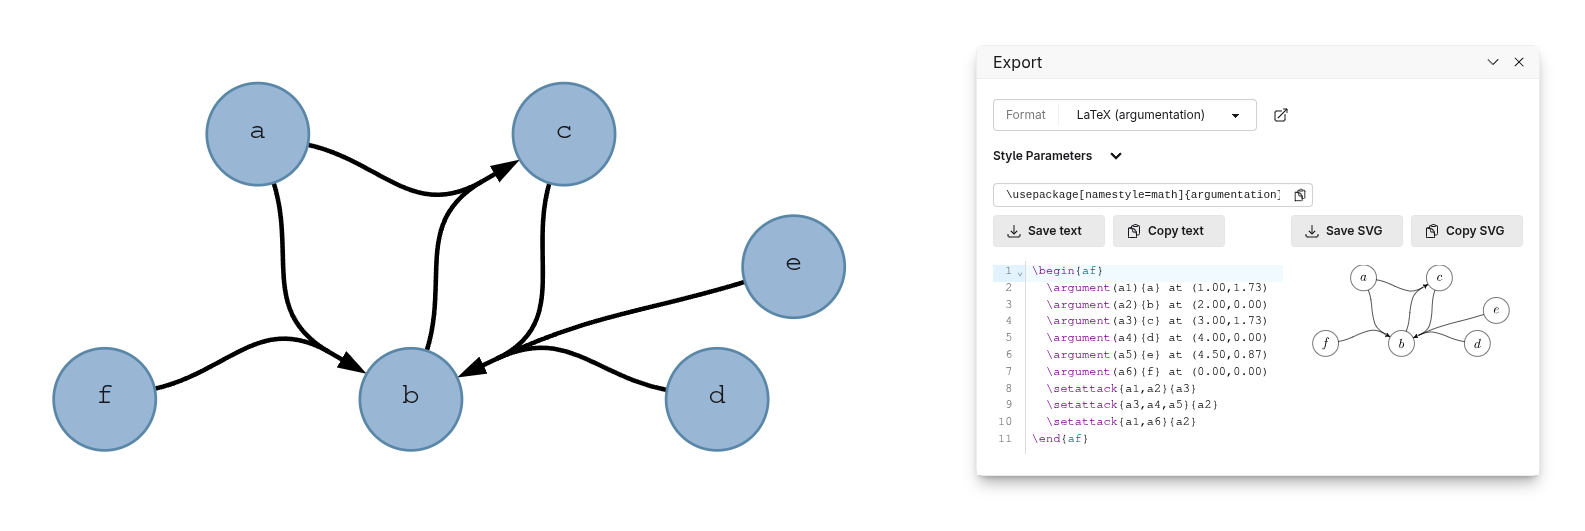
\includegraphics[width=0.93\linewidth]{figures/screenshot-setaf.png}\\[0.6ex]
        \raggedright\footnotesize
        \textbf{Collective attacks \& export (SetAF).} A \emph{set} of arguments jointly
        attacks a target, drawn as hyperedges; the export window emits ready-to-use
        \LaTeX{} with an SVG preview.
    \end{minipage}
}
\end{columns}

%======================================================================
% Row 5 — Semantics + Outlook
%======================================================================
\begin{columns}
\column{0.58}
\block{Supported Semantics}{
    \small
    \renewcommand{\arraystretch}{1.25}
    \begin{tabular}{@{}p{0.30\linewidth}p{0.64\linewidth}@{}}
        \toprule
        \textbf{Group} & \textbf{Semantics}\\
        \midrule
        Classical & conflict-free, admissible, complete, grounded, preferred, stable\\
        Admissibility-based & ideal, semi-stable, eager, strong admissibility, initial sets, unchallenged\\
        Non-admissible & naive, CF2, SCF2, stage, stage2, (strongly) undisputed\\
        Weak-admissible & w-admissible, w-complete, w-grounded, w-preferred\\
        \midrule
        Rankings & burden, categoriser, counting, discussion, iterated graded defense, serialisability, social, strategy, tuples\\
        \bottomrule
    \end{tabular}

    \vspace{0.8ex}
    {\footnotesize Available across AF, BAF, iAF, PAF and SetAF; ADFs use the three-valued
    classical and naive semantics. Serialisation sequences are supported interactively.}
}
\column{0.42}
\useblockstyle{aigposterblockY}
\block{Outlook}{
    \vspace{0.2cm}
    Planned extensions:
    \begin{itemize}\setlength{\itemsep}{0.5ex}
        \item further formalisms --- Assumption-Based Argumentation, Weighted AFs, Bipolar
        Set-based AFs, claim-augmented AFs;
        \item benchmark generators from the ICCMA ecosystem;
        \item explanation-based reasoning: \emph{why} is an argument accepted?
    \end{itemize}
    \vspace{0.3cm}
    \yellowhighlight{\parbox{0.96\linewidth}{\vspace{0.3ex}\centering
    \agon is backend-agnostic and open to new formalisms and solvers.\vspace{0.3ex}}}
}\useblockstyle{aigposterblockB}
\end{columns}

%======================================================================
% Footer
%======================================================================
\begin{columns}
\column{1.0}
\block{}{
    \centering
    {\large
    \textbf{Live:}~\texttt{agon.tweetyproject.org} \quad$\bullet$\quad
    \textbf{Source:}~\texttt{github.com/aig-hagen/AgonProject} \quad$\bullet$\quad
    GPL-3.0}\\[0.6ex]
    {\footnotesize Partially supported by the Deutsche Forschungsgemeinschaft (project
    ``Argumentative Reasoning in Nonsensical Situations'', ARNS, grant 550735820).}
}
\end{columns}

\end{document}
